\documentclass[a4paper]{report}
\usepackage{apacite}
\usepackage{graphicx}
\usepackage{algorithm}
\usepackage{algcompatible}
\usepackage[section]{placeins}
\graphicspath{{Images/}}
\setlength\parindent{0pt}

\makeatletter
\AtBeginDocument{%
	\expandafter\renewcommand\expandafter\subsection\expandafter{%
		\expandafter\@fb@secFB\subsection
	}%
}
\makeatother

\begin{document}
	%------------------------Cover-------------------------------------------------------------
	\begin{titlepage} 
		\newcommand{\HRule}{\rule{\linewidth}{0.5mm}}
		
		\center 
		
		\textsc{\large Project 1.1 - Block 3}\\[0.5cm] 
		
		\HRule\\[0.4cm]
		
		{\huge\bfseries Compute chromatic numbers}\\[0.4cm] 
		
		\HRule\\[1.5cm]
		
		\textsc{\large Group 10}\\[0.5cm]

		\begin{minipage}{0.6\textwidth}
			\begin{flushleft}
				Tu Anh Dinh\\Michal Jarski\\Vaishnavi Velaga
			\end{flushleft}
		\end{minipage}
		~
		\begin{minipage}{0.3\textwidth}
			\begin{flushleft}
				Rudy Wessels\\Oskar Wielgos\\
			\end{flushleft}
		\end{minipage}
		
		\vspace{2cm}
		
		Submitted: Wednesday January 23, 2019
		
		
	\end{titlepage}
	
	
	
	
	
	%-------------------Title page-----------------------------------------------------------
	\begin{titlepage} 
		\newcommand{\HRule}{\rule{\linewidth}{0.5mm}} 
		
		\center
		
		\textsc{\LARGE Maastricht University}\\[1.5cm]
		
		\textsc{\Large Department of Data Science and Knowledge Engineering}\\[0.5cm] 
		
		\textsc{\large Project 1.1 - Block 3}\\[0.5cm] 
		
		\HRule\\[0.4cm]
		
		{\huge\bfseries Compute chromatic numbers}\\[0.4cm] 
		
		\HRule\\[1.5cm]
		
		\textsc{\large Group 10}\\[0.5cm]
		
		\begin{minipage}{0.6\textwidth}
			\begin{flushleft}
				Tu Anh Dinh\\Michal Jarski\\Vaishnavi Velaga
			\end{flushleft}
		\end{minipage}
		~
		\begin{minipage}{0.3\textwidth}
			\begin{flushleft}
				Rudy Wessels\\Oskar Wielgos\\
			\end{flushleft}
		\end{minipage}
	
		 \vspace{1cm}
		Submitted: Wednesday January 23, 2019
		\vspace{3cm}
		\begin{flushleft}
			Project coordinator: Prof. Jan Paredis
		\end{flushleft}
		
	\end{titlepage}
	
	%-----------------------------------------------------------------------------
	\chapter*{Preface}
	\pagenumbering{gobble}

	\addcontentsline{toc}{chapter}{Preface}
	This report is the outcome of group 10's work for project 1.1: Graph Coloring. It can be used as a guideline to partially solve the NP-complete problem of finding the chromatic number of a graph.
	  
	
	%-----------------------------------------------------------------------------
	\chapter*{Summary}
	\addcontentsline{toc}{chapter}{Summary}
	The chromatic number of a graph is the minimum number of colors needed to color the vertices of the graph such that no two adjacent vertices share the same color. Finding the chromatic number of a graph is a NP-complete problem, which has many applications such as automated timetabling and scheduling. This project solves the problem of finding the smallest range of the chromatic number of a graph. We propose an approach that combines different methods such as graph decomposition, greedy algorithms, identifying special cases of graphs, a brute-force algorithm and genetic algorithm. The proposed approach is analyzed on a set of 20 graphs. It gives decent results on graphs with special structures, even if the graphs' sizes are big. For large graphs without special structures, the results are unpredictable. 
	
	%-----------------------------------------------------------------------------
	\tableofcontents
	
%	\chapter*{Abbreviations and symbols}
%	\addcontentsline{toc}{chapter}{List of abbreviations and symbols}

	
	%-----------------------------------------------------------------------------
	\chapter{Introduction}
	\pagenumbering{arabic}
	As stated above, the chromatic number of a graph is the minimum number of colors needed to color the vertices of the graph such that no two adjacent vertices share the same color. In this project, we provide an approach to find the smallest range of the chromatic number of a graph. \\
	
	The problem description is as follows. Given a graph G=(V,E) where V is the set of vertices and E is the set of edges that connect the vertices. In this project, the input graphs are undirected graph, where the edges have no orientation. In addition, a vertex must not connect to itself and the number of edges between two vertices must not exceed 1.  Graph coloring is coloring the vertices of a graph such that no two adjacent vertices share the same color. Graph coloring is one of the important topics of graph theory and is used in various research areas of computer science such as data mining and networking.\\
	The smallest number of colors used in graph coloring is called the chromatic number. A lower bound of a graph is a number that is less than or equal to the chromtic number, while an upper bound is a number that is greater than or equal to the chromtic number. The purpose of this project is to find the closest upper bound, lower bound and, if possible, the chromatic number of a graph.\\
	
	The approach proposed for this project is combining different methods such as graph decomposition, greedy algorithms, identifying special cases of graphs, a brute-force algorithm and genetic algorithm. A greedy algorithm is used to find the lower bounds; while another greedy algorithm and the genetic algorithm are used to find the upper bounds. Algorithms for testing special cases and brute-force algorithm are used to find the chromatic numbers if possible. Graph decomposition helps impove the execution time and the results of other methods. The approach is then analyzed on a set of 20 graphs, where the structure of each graph is exploited to see the correlation between the types of graphs and the results on those graphs. The approach gives decent results on graphs with special structures, even if the graphs' sizes are big. For large graphs without special structures, the results are unpredictable. \\

	The rest of the report is divided as follows. Chapter 2 is about the methods used to compute the upper bound, lower bound and the chromatic number of a graph. Different algorithms are used: graph decomposition, greedy algorithm, identifying special cases of graphs, brute-force algorithm and genetic algorithm. Chapters 3,4 and 5 are about experiments and their results. The last chapter gives the conclusion for the project.
	
	\chapter{Methods}
	This chapter describes the approach used for finding the lower bound, upper bound and if possible, the chromatic number of a graph. 
	\section{Overview}
	The proposed approach in this report is a combination of different methods. Since the execution time is normally limited, methods that give out results fast are executed first. Algorithm \ref{alg:overview} describes the general work flow.\\
	\begin{algorithm}
		\caption{General work flow}
		\label{alg:overview}
		\begin{algorithmic}[1]
			\REQUIRE a graph
			\STATE upperbound = greedyUpperbound(graph)
			\STATE components = decompose(graph)
			\FORALL{components} 
				
				\IF{component is special case} 
					\STATE chromaticNumber of component = chromaticNumber of special case
					\STATE Go to the next component
				\ELSE 
					\STATE componentLowerbound = 3
				\ENDIF
				
				\IF{greedyLowerbound(component) $>$ 3}
				\STATE componentLowerbound = greedyLowerbound(component)
				\ENDIF
				
				\STATE componentUpperbound =  greedyUpperbound(component)

				\IF{componentUpperbound = componentLowerbound} 
				\STATE chromaticNumber of component = componentUpperbound
				\STATE Go to the next component
				\ENDIF
				
				\IF{number of vertices $<=$ 20} 
				\STATE chromaticNumber of component = BruteForce(component)
				\ENDIF 
			\ENDFOR

			\STATE newUpperbound = max(upper bounds of components)
			
			\IF{newUpperbound $<$ upperbound} 
			\STATE upperbound = newUpperbound 
			\ENDIF
			
			\STATE lowerbound = max(lower bounds of components)
			
			\IF{has found all chromatic numbers of components} 
			\STATE chromatic number = max(chromatic numbers of components)
			\ELSE
			\STATE lowerbound = max(chromatic numbers of components)
			\ENDIF
			
			\STATE geneticAlgorithm(graph)
		\end{algorithmic}
	\end{algorithm}
	The proposed approach works as follows. First, a greedy algorithm calculates the upper bound of the given graph (line 1). Then, the given graph is decomposed into connected components. Each component is checked to see if it is one of the special cases where the chromatic number can be concluded immediately (line 3 - 7). The special cases are listed below: 
	\begin{itemize}
		\item No-vertex graph: chromatic number is 0
		\item No-edge graph: chromatic number is 1
		\item Bipartite graph: chromatic number is 2
		\item Odd cycle graph: chromatic number is 3
		\item Complete graph: chromatic number is the number of vertices
	\end{itemize}
	In line 8, if a component is none of the special cases then a lower bound of the component is 3, since the first three cases have covered all graphs with chromatic number below 3. It is then compared to the lower bound computed by a greedy algorithm to update the bigger lower bound (line 10 - 12). \\
	Then an upper bound of the component is computed by another greedy algorithm (line 13). The reason for running the greedy algorithm for upper bound on both the original graph and its components is that the result upper bounds are sometimes different, so we run both on the original graph and its components to increase the chance that a better upper bound is found.  However, the greedy algorithm for lower bound normally gives the same results after running on both the original graph and its components, so it is run only on the components. \\
	Next, if the lower bound and upper bound are equal, then the chromatic number can be concluded (line 14 - 17). \\
	If the chromatic number of a component still cannot be calculated then a brute-force algorithm is used (line 18 - 20). However, only components with number of vertices below 20 are proccessed with the brute-force algorithm, since the brute-force algorithm normally takes long to execute on bigger graphs. Without time-restriction, the more time we have, the higher the threshold for brute-force can be (about 30 to 40).\\
	
	After proccessing on the components, the upper bound, the lower bound and possibly the chromatic number of the original graph can be concluded. The biggest upper bound among the components is a upper bound of the original graph (line 22). This new upper bound is then compared to the previously computed upper bound in line 1 to output the better one. Similarily, the biggest lower bound among the components is a lower bound of the original graph (line 26). \\
	If the chromatic numbers of all components have been found, then the chromatic number of the original graph is the biggest chromatic number among those of the components (line 27 - 29). If it is not the case, then the biggest chromatic number found on the components is another lower bound for the original graph (line 30).\\
	Finally, in line 32, genetic algorithm is used to bring the upper bound closer to the chromatic number. Genetic algorithm is run last because there is no guarantee on its execution time.\\
	
	The algorithm for each method is described in the next sections of this chapter.
	

		\section{Graph decomposition}
		One graph can contain multiple disconnected parts, which can be considered as independent subgraphs (Figure \ref{fig:decompose}). Graph decomposition means seperating the graph into fully connected components. Decomposing the graph will allow other methods to work on smaller graphs. Algorithm \ref{alg:decompose} describes the method for decomposing a graph into components.\\
		
		\begin{figure}[h]
			\centering
			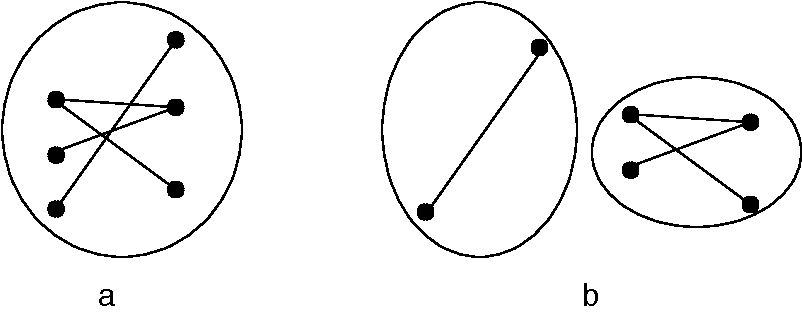
\includegraphics[width=50mm,scale=0.5]{figures/DecomposedGraph.pdf}
			\caption{A graph (a) before decomposed and (b) after decomposed}
			\label{fig:decompose}
		\end{figure}
	
		\begin{algorithm}
			\caption{Decomposing a graph}
			\label{alg:decompose}
			\begin{algorithmic}[1]
				\REQUIRE a graph
				\STATE Create listOfVertices 
				\STATE listOfVertices.add(all vertices in the graph)
				\WHILE{listOfVertices is not empty}
				\STATE Create a new component
				\STATE Create a new uncheckedList
				\STATE component.add(firstVertex in listOfVertices )
				\STATE uncheckedList.add(firstVertex in listOfVertices)
				\STATE listOfVertices.remove(first element)
				\WHILE{uncheckedList is not empty} 
				\STATE checkingVertex = first vertex in the uncheckedList
				\FORALL{neighbors of checkingVertex} 
				\IF{neighbor is not in component} 
				\STATE uncheckedList.add(neighbor)
				\STATE component.add(neighbor)
				\ENDIF
				\STATE listOfVertices.remove(neighbor)
				\ENDFOR
				\STATE Remove checkingVertex from uncheckedList
				\ENDWHILE
				\STATE Convert component to standard form
				\STATE components.add(component)
				\ENDWHILE
				\STATE \textbf{return} components
				
			\end{algorithmic}
		\end{algorithm}
		The proposed graph decomposition algorithm is based on breadth-first search. A unchecked-list stores the vertices whose neighbors are not yet added to the current expanding component. In line 6 and 7 the first vertex is added to a component and the unchecked list. Then all the neighbors of the vertex are added to the component and the unchecked list, and the first vertex of the unchecked list is removed (line 9 - 19). To avoid loops, only vertices not in the component are added. The same is done for all vertices in the unchecked list, until the list is empty. The process is repeated until all vertices in the original graph are classified into components.\\
		
		Note that the vertices of the input graphs in this project are represented by successive numbers. All algorithms are implemented based on this data structure. Therefore, after classifying the vertices into components, each component is then converted to the standard form, where the indexes of vertices are successive numbers (line 20).
		
		\section{Greedy algorithm for upper bound}
		Greedy algorithm for upper bound provides an efficient way of coloring a graph, with short execution time. However, it does not guarantee that the coloring is optimal. Therefore, it can be used to calculate a upper bound. Algorithm \ref{alg:greedy} \cite{jensen2011graph} describes this method.\\
		\begin{algorithm}
			\caption{Greedy algorithm for upper bound}
			\label{alg:greedy}
			\begin{algorithmic}[1]
				\REQUIRE a graph
				\STATE Sort vertices in non-increasing order of degrees (the number of neighbors)
				\STATE Create availableColors list
				\FORALL{vertices}
					\FORALL{colors in availableColors}
					\IF{color is valid for vertex}
					\STATE Assign the color for the vertex
					\STATE break
					\ENDIF
					\ENDFOR
					\IF{The vertex is still not colored}
					\STATE Create a new color
					\STATE Assign the new color for the vertex
					\STATE Add the new color to availableColors list
					\ENDIF
				\ENDFOR
				\STATE \textbf{return} size of availableColors list
			\end{algorithmic}
		\end{algorithm}
		First, the vertices are sorted based on their degrees (line 1). The degree of a vertex is the number of other vertices connected to that vertex. The vertex with higher degree will be colored first.\\
		When coloring a vertex, the available colors is reused as much as possible (line 4-9). If none of the available colors is valid to color that vertex, then a new color is generated and added to the available list (line 10-14). When the graph is fully colored, the number of colors in the available list is returned as an upper bound.\\
		
		\section{Greedy algorithm for lower bound}
		A greedy algorithm is used to find several cliques in a graph and returns the size of the biggest clique found \cite{steven2008algorithm}. The biggest size is then return as a lower bound. However, it does not guarantee to find the maximum clique. \\
		
		The algorithm works as follows. To form a clique, an initial vertex is added to the clique. Then, for every other vertex, we add it to the clique if it is connected to all vertices currently in the clique. The same proccess is repeated to find multiple cliques, where every vertex in the original graph is used as the initial vertex for a clique. \\
		
		Even though the algorithm does not guarantee to find the maximum clique, it is still promissing that the algorithm will find cliques that are big compared to the graphs' sizes. Since the algorithm goes through every vertex in the graph and forms a clique that contains the vertex, the bigger the clique is, the better chance that it can be found.
		
		\section{Special cases}
			\subsection{Bipartite}
			A bipartite graph is a graph which its vertices can be separated into two sets such that there is no connection between any pair of vertices of the same set.\\
			The chromatic number of a bipartite graph is 2. Algorithm \ref{alg:bipartite} \cite{sedgewick2003} describes the steps to test whether a graph is bipartite, using breadth-first search. \\
			
			\begin{figure}[h]
				\centering
				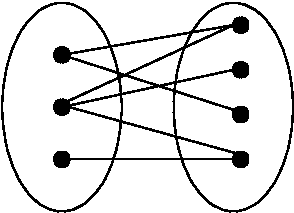
\includegraphics[width=50mm,scale=0.5]{figures/bipartite.pdf}
				\caption{An example of bipartite graphs}
				\label{fig:bipartite}
			\end{figure}
			
			\begin{algorithm}
				\caption{Bipartite testing}
				\label{alg:bipartite}
			
				\begin{algorithmic}[1]
					\REQUIRE a graph
					\STATE Create unchecked list
					\STATE unchecked.add(first vertex)
					\STATE Assign one color to the first vertex
					\WHILE{The graph is not fully colored}
					\WHILE{unchecked list is not empty}
					\STATE checkingVertex = unchecked.getFirstElement()
					\STATE unchecked.removeFistElement()
					\FORALL{neighbors of checkingVertex}
					\IF{neibor not yet colored}
					\STATE Assign the opposite color of checkingVertex's color to neighbor
					\STATE unchecked.add(neighbor)
					\ELSIF{neighbor has invalid color}
					\STATE \textbf{return} false
					\ENDIF
					\ENDFOR
					\ENDWHILE
					\ENDWHILE
					\STATE \textbf{return} true
				\end{algorithmic}
			\end{algorithm}
			 Two colors are used to color the graph. A unchecked list stores the vertices whose neighbors are not yet considered. First, one color is assigned to the first vertex and the first vertex is added to the unchecked list (line 2-3). Then, all its neighbors are considered and the vertex itself is removed from the unchecked list. For each neighbor, if the neighbor has not been colored then it is assigned with the oposite color (line 10). If the neighbor has been colored, then we check if it is a valid coloring. If the coloring is invalid, the graph is not bipartite (line 12-13). The same is done for all elements in the unchecked list, until the list is empty. The process is repeated until all vertices in the graph are colored. If the graph is successfully colored, then it is bipartite.
			\subsection{Odd cycle}
			An odd cycle is a cycle with an odd number of edges and vertices (Figure \ref{fig:oddcycle}). The chromatic number of an odd cycle graph is 3. \\
			
			\begin{figure}[h]
				\centering
				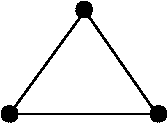
\includegraphics[width=50mm,scale=0.5]{figures/cycle.pdf}
				\caption{An example of odd cycle graphs}
				\label{fig:oddcycle}
			\end{figure}
		
			The method for testing if a graph is an odd cycle checks for three condition:
			\begin{itemize}
				\item The number of vertices is equal to the number of edges
				\item Every vertex has two neighbors
				\item The number of vertices is odd
			\end{itemize}
			A graph is an odd cycle graph if and only if all three conditions are satisfied.
			
			\subsection{Complete graph}
			A complete graph (Figure \ref{fig:complete}) is a graph where every vertex is connected to all other vertices. The chromatic number of a complete graph is the number of vertices. The method checks weather a graph has the above conditions to determine if it is a complete graph.
			\begin{figure}[h]
				\centering
				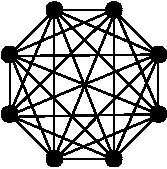
\includegraphics[width=50mm,scale=0.5]{figures/complete.pdf}
				\caption{An example of complete graphs}
				\label{fig:complete}
			\end{figure}
			
		\section{Brute-force algorithm}
		The brute-force algorithm simply generates every possible coloring and checks if it is a valid one. In case the coloring is valid, the algorithm terminates with a possibilty of returning an array of colors assigned to each node and the chromatic number. In order to check the validity of coloring, it utilizes isValid algorithm, which iterates through the array representing nodes' colors and searches for a conflict (two adjacent/connected nodes assigned the same color). If a conflict is found, the method returns false, meaning certain coloring is not a valid one.\\
		
		Brute-force is based on raw computetional power, thus making it heavily dependent on the hardware that runs it. Finding the chromatic number is guaranteed sooner or later. However in reality, its use is limited to graphs not bigger than 20 vertices, and even then, depending yet on how the vertices are being connected.\\
		
		Algorithms calculating lower bound or applying pruning, might futher optimize it, reducing the time needed to find the chromatic number. \\
		
		Implementing a greedy-type brute-force could also bring significant improvements on effectiveness and execution time, but on the other hand, causing a risk of omitting the right coloring and eventually not finding the chromatic number, but only its approximation.	
			
		\section{Genetic algorithm}
%			\subsection{Fitness function}
%			\subsection{Selection method}
%			\subsection{Crossover}
%			\subsection{Mutation}
		The genetic algorithm is an algorithm for calculating the upper bound together with working its way down to finding lower and better upper bounds for a particular graph. It starts with creating a population of individuals each containing a randomly colored version of the selected graph. The size of this population can be set to any number preferred. Once the population is created it assigns a fitness (which is a real number between 0 and 1) to each individual based on the number of incorrect edges. Following up the individuals are sorted by fitness from high to low (1$>$0), at which it becomes clear what part of the population has the highest correctness of coloring.\\
		
		After the individuals are sorted the selection method picks out the “parents” for the next generation through an elitist approach. These parents are utilized for the crossover method creating combinations of two of the parents until there are enough new individuals for the next generation with equal size to the previous one. Afterward, the mutation method, depending on the extent of the mutation rate, will mutate some individuals’ coloring of the graph to achieve possibly better results. By results is meant, individuals with higher fitness.
\\
		
		Lastly, this process runs over several generations/populations through a loop till the algorithm finds an individual with fitness “1” (no incorrect edges). When this is the case, the new upper bound will be printed in the command prompt based on how many colors were used to achieve this solution. Following up the entire process starts over with one less color, so that the upper bound will be lower after each successful finding.
		
		
		
	\chapter{Experiments}
	The experiments are set up to run on the given 20 graphs from phase 3 of the project. Each graph is exploited to see the following properties:
	\begin{itemize}
		\item The number of vertices (or the size of the graph)
		\item The number of connected components
		\item The size of each component
		\item The number of components that are special cases
		\item The biggest clique found
	\end{itemize}

	\chapter{Results}
	This chapter represents the results of the proposed approach on the given 20 graphs from phase 3 of the project. Table \ref{tab:result} shows the upper bounds, lower bounds and chromatic numbers found on the graphs, while table \ref{tab:prop} shows the properties of the graphs.
		\begin{table} [h!]
		\begin{center}
			\begin{tabular}{| c | c | c | c |c|}
				\hline
				Graph no. & Upper bound & Lower bound & Chromatic number & Gap \\
				\hline
				1 & 3 & $-$ & 3 & 0\\
				\hline
				2 & 5 & 3 & $-$ & 2\\
				\hline
				3 & 8 & 6 & $-$ & 2\\
				\hline
				4 & 7 & 4 & $-$ & 3\\
				\hline
				5 & 2 & $-$ & 2 & 0\\
				\hline
				6 & 3 & $-$ & 3 & 0\\
				\hline
				7 & 12 & 8 & $-$ & 4\\
				\hline
				8 & 98 & $-$ & 98 & 0\\
				\hline
				9 & 6 & 3 & $-$ & 3\\
				\hline
				10 & 3 & $-$ & 3 & 0\\
				\hline
				11 & 15 & 15 & 15 & 0\\
				\hline
				12 & 2 & $-$ & 2 & 0\\
				\hline
				13 & 14 & 9 & $-$ & 5\\
				\hline
				14 & 5 & 3 & $-$ & 2\\
				\hline
				15 & 10 & 5 & $-$ & 5\\
				\hline
				16 & 4 & 3 & $-$ & 1\\
				\hline
				17 & 8 & $-$ & 8 & 0\\
				\hline
				18 & 11 & 10 & $-$ & 1\\
				\hline
				19 & 11 & 11 & 11 & 0\\
				\hline
				20 & 9 & 8 & $-$ & 1\\
				\hline
			\end{tabular}
		\end{center}
		\caption{Results on the given 20 graphs from phase 3. The column "Gap" represents the differences between upper bounds and lower bounds}
		\label{tab:result}
	\end{table}
	
	\begin{table} [h!]
		\begin{center}
			\centerline{
			\begin{tabular}{| c | c | c | c |c|c|c|}
				\hline
				Graph no. & Size & \shortstack{Number of \\ components}& Components' sizes & Special cases&\shortstack{Biggest clique\\ found}& Gap \\
				\hline
				1 & 212 & 1 & 212 &0&3& 0\\
				\hline
				2 & 456 & 8 & 448, 2, 1 (6 times) &7&3& 2\\
				\hline
				3 & 218 & 2 & 212, 6 &1&3& 2\\
				\hline
				4 & 107 & 1 & 107 &0&4& 3\\
				\hline
				5 & 4007 & 1 & 4007 &1&$-$& 0\\
				\hline
				6 & 529 & 260 & 8, 5, 2 (258 times) &260&$-$& 0\\
				\hline
				7 & 43 & 1 & 43 &0&8& 4\\
				\hline
				8 & 107 & 1 & 107 &0&98& 0\\
				\hline
				9 & 206 & 1 & 206 &0&3& 3\\
				\hline
				10 & 166 & 1 & 166 &0&2& 0\\
				\hline
				11 & 164 & 1 & 164 &0&15& 0\\
				\hline
				12 & 744 & 1 & 744 &1&$-$& 0\\
				\hline
				13 & 85 & 1 & 85 &0&9& 5\\
				\hline
				14 & 907 & 1 & 907 &0&3& 2\\
				\hline
				15 & 215 & 1 & 215 &0&5& 5\\
				\hline
				16 & 164 & 1 & 164 &0&2& 1\\
				\hline
				17 & 106 & 12 & 92, 2, 3, 1 (9 times) &11&8& 0\\
				\hline
				18 & 131 & 5 & 26 (2 times), 25 (2 times), 29 &0&10& 1\\
				\hline
				19 & 143 & 1 & 143 &0&11& 0\\
				\hline
				20 & 387 & 1 & 387 &0&8& 1\\
				\hline
			\end{tabular}
		}
		\end{center}
		\caption{Properties of the given 20 graphs from phase 3, along with the gaps between upper bounds and lower bounds found}
		\label{tab:prop}
	\end{table}
	\chapter{Discussion}
	As can be seen from the results, our algorithms perform well to find the chromatic numbers of several types of graphs:
	\begin{itemize}
		\item For graphs that are special cases, the chromatic numbers can be found quickly, even if the graphs' sizes are large. For example, the sizes of graph 5 and graph 12 are 4007 and 744 respectively, but since they are bipartite graphs, their chromatic numbers were found in less than 1 minute. The reason for this is that the time complexities of special cases testing algorithms are low, as mentioned in chapter 2.
		\item For graphs that are disconnected, the algorithm also gives good results. For example, graph 2, 3, 6, and 17 can be decomposed into 8, 2, 260, 12 and 5 components respectively, so their ranges for chromatic numbers are small (less than or equal to 2).
		\item For graphs that have big clique sizes compared to the graphs' sizes, the gaps between the upper bounds and lower bounds found are small. For example, graph 8 has the size of 107 and the biggest clique size found is 98, so our algorithms can find its chromatic number. This is an example which proves that the bigger the clique is, the more likely it can be found, as stated in chapter 2.
	\end{itemize}
	On the other hand, the algorithms do not give good results on certain graphs that do not have special structures. For example, graph 13 and 15 are fully connected, they are none of the special cases and their biggest clique sizes found are small compared to the graphs' sizes. Therefore, their ranges for chromatic number are higher (where the differences between upper bounds and lower bounds are both 5).
	
	\chapter{Conclusion}
	In this project, the problem of finding chromatic number for a graph is partially solved. This is a NP complete problem, so the approach is to use multiple combined algorithms to find the smallest range for the chromatic number. A greedy algorithm is used to find the lower bounds; while another greedy algorithm and the genetic algorithm are used to find the upper bounds. Algorithms for testing special cases and brute-force algorithm are used to find the chromatic numbers if possible. Graph decomposition helps impove the execution time and the results of other methods. \\
	
	The approach is analyzed on a set of 20 graphs, where the structure of each graph is exploited to see the correlation between the types of graphs and the results on those graphs. The approach gives decent results on graphs with special structures, even if the graphs' sizes are big. For large graphs without special structures, the results are unpredictable. \\
	
	The results from the experiments give insights into the proposed approach. Greedy algorithms often give decent results with short execution time, but do not guarantee the optimal results. On the other hand, brute-force algorithm guarantees the optimal results, but has high complexity, therefore it can only be used on graphs with small number of vertices. Genetic algorithm normally gives better results than greedy algorithm, but the execution time is longer, and the results are also not guaranteed to be optimal. Special cases testing algorithms such as bipartite testing, complete graph testing have low complexity, thus they can give out the results fast. However, the use of special cases testing algorithms are limited on graphs with special structures. \\
	
	The approach proposed in this report can be used as a starting point for solving the graph coloring problem. More enhanced methods such as linear programming or constraint satisfaction can be used for further research.
	
	\bibliographystyle{apacite}
	\bibliography{references}
	
%	\appendix
%	\chapter*{Appendix}
%	\addcontentsline{toc}{chapter}{Appendix}
\end{document}